\documentclass[11pt]{beamer}
\RequirePackage{etex}

\let\Tiny=\tiny

\usefonttheme[onlymath]{serif}

\usepackage{color}
\usepackage{colortbl}
\usepackage{multicol}
\usepackage{amssymb,amsmath,amsthm,stmaryrd}
\usepackage{indentfirst}
\usepackage{latexsym}
\usepackage[utf8]{inputenc}
\usepackage{fancybox}
\usepackage{tikz}
\usepackage{tikz-qtree}
\usepackage{eurosym}
\usepackage{listings}
\usepackage{soul}
\usepackage{upquote}
\usepackage{cancel}
\usepackage{xfrac}
\usepackage{tkz-graph}  
\usepackage{dirtree}

\definecolor{light_red}{rgb}{1,0.95,0.95} 
\definecolor{gray}{rgb}{0.5,0.5,0.5} 
\definecolor{green}{rgb}{0.05,0.4,0.25} 

\newcommand{\system}[1]{{\color{red}\texttt{S: #1}}\\}
\newcommand{\user}[1]{{\color{teal}\texttt{U: #1}}\\}
\newcommand{\comment}[1]{{\color{orange}\texttt{#1}}\\}

\usetikzlibrary{trees,shapes,decorations}
\usetikzlibrary{shapes.geometric}

\setbeamertemplate{navigation symbols}{}
\setbeamercovered{transparent}

\title[Fluency project tutorial]{Fluency project tutorial}
\author{Jose F Quesada \& Jose Luis Pro}
\date{}

\mode<presentation>{\usetheme[]{Warsaw}}

\setbeamertemplate{footline}
    {
      \leavevmode
      \hbox{\begin{beamercolorbox}[wd=.5\paperwidth,ht=2.5ex,dp=1.125ex,leftskip=.3cm plus1fill,rightskip=.3cm]{author in head/foot}
        \usebeamerfont{author in head/foot}\insertshorttitle%
      \end{beamercolorbox}%
      \begin{beamercolorbox}[wd=.5\paperwidth,ht=2.5ex,dp=1.125ex,leftskip=.3cm,rightskip=.3cm plus1fil]{title in head/foot}
        \usebeamerfont{title in head/foot}
					\hfill\insertframenumber\,/\,\inserttotalframenumber
      \end{beamercolorbox}}
      \vskip0pt
    }

\hypersetup{pdfpagemode=UseNone}

\newcommand{\Operator}[1]{\textcolor{green}{#1}}

\lstset
{
	basicstyle=\ttfamily,
	keywordstyle=\color{blue}\ttfamily,
  stringstyle=\color{red}\ttfamily,
  commentstyle=\color{green}\ttfamily,
  language=C,                			% choose the language of the code
  numbers=left,                   % where to put the line-numbers
  stepnumber=1,                   % the step between two line-numbers.        
  numbersep=5pt,                  % how far the line-numbers are from the code
  backgroundcolor=\color{white},  % choose the background color. You must add \usepackage{color}
  showspaces=false,               % show spaces adding particular underscores
  showstringspaces=false,         % underline spaces within strings
  showtabs=false,                 % show tabs within strings adding particular underscores
  tabsize=3,                      % sets default tabsize to 3 spaces
  captionpos=b,                   % sets the caption-position to bottom
  breaklines=true,                % sets automatic line breaking
  breakatwhitespace=true,         % sets if automatic breaks should only happen at whitespace
}

\lstdefinelanguage{lekta}
{
	language=C,
	backgroundcolor=\color{light_red},
	numberstyle=\tiny\color{gray},
	morekeywords=
	{
		classDef,
		Void,
		cond,
		boolean,
		String,
		True,
		False,
		\#Include,
	},
	alsoletter={\#},
	literate= {->}{{\Operator{->}}}1
						{>>}{{\Operator{>>}}}1
						{\&\&}{{\Operator{\&\&}}}1
						,	
	keywordstyle=[2]\color{purple},
	keywords=[2]
	{
		lektaProject,
		projectHead,
		projectLanguageScope,
		projectCompileOutput,
		projectSetup,
		setupParserRoots,
		classModel,
		lexicalModel,
		forLanguage,
		grammaticalModel,
		LaunchLektaKernel,
		UseProject,
		ProjectCompile,
		DisplayProcessUnderstandingOn,
		CreateDialogue,
		ElementBool,
		ElementInt,
		ElementReal,
		ElementLiteral,
		ElementRange,
		StructureBatch,
		StructureComplex,
		Synonym,
		MindBoardStructure,
		conversationalModel,
		ColligoSchemata,
		ColligoCapture,
		ColligoScheme,
		ColligoAction,
		SensoSchemata,
		SensoScheme,
		SensoCapture,
		SensoAction,
		CogitoScheme,
		CogitoCapture,
		CogitoAction,
		CogitoSchemata,
		RespondoSchemata,
		RespondoScheme,
		RespondoCapture,
		RespondoAction,
		LocutioSchemata,
		LocutioScheme,
		LocutioCapture,
		LocutioAction,
		scriboModel,
		ScriboSchemata,
		ScriboScheme,
		ScriboCapture,
		ScriboAction,
	},
}

\begin{document}

\begin{frame}
\titlepage
\end{frame}

\section{Project motivation}

\begin{frame}
\frametitle{Current state}
	\setbeamercolor{block title}{use=structure,fg=white,bg=red!75!black}
	\setbeamercolor{block body}{use=structure,fg=black,bg=red!10!white}
	\begin{block}{What do we have now?}
			\begin{itemize}
				\item With lekta we can create dialogue systems based upon a certain domain.
				\item We create lexicons, grammar rules, mind structures and generation strategies in order to get that domain fully implemented.
				\item But all that things are created \emph{ad-hoc} for that domain.
				\item If we want to implement another different dialogue system we must start again.
				\item Without being possible to reuse lexicons or grammar rules.
				\item It's necessary to have a good level in programming skills and some experience in the implementation of grammars.
			\end{itemize}
	\end{block}
\end{frame}

\begin{frame}
\frametitle{Dialogue systems implemented in the exercises}
	\setbeamercolor{block title}{use=structure,fg=white,bg=green!75!black}
	\setbeamercolor{block body}{use=structure,fg=black,bg=green!10!white}
	\begin{block}{Examples}
			\begin{itemize}
				\item Session 04: Exercise 01.
				\begin{itemize}
					\item In integer calculator exercise we have ``english numbers'' grammar. 
					\item But mind structure was an ``Expression object'' (not reusable).
				\end{itemize}
				\vspace{15pt}
				\pause
				\item Session 04: Exercise 02.	
				\begin{itemize}
					\item In domotics assistant exercise we had grammars and lexicon for actions and devices. 
					\item And mind structures were basically boolean flags to represent devices context state.
				\end{itemize}
			\end{itemize}
	\end{block}
\end{frame}

\begin{frame}
	\setbeamercolor{block title}{use=structure,fg=white,bg=red!75!black}
	\setbeamercolor{block body}{use=structure,fg=black,bg=red!10!white}
	\begin{block}{What do we want?}
			\begin{itemize}
				\item \textbf{General purpose DM:} We would like a dialogue manager reasoning engine domain-independent.
				\item \textbf{Reusability:} Grammar for some parameters should be reusable. For example, a grammar for english dates or numbers can be used in all imaginable domains with almost no difference between them.
				\item \textbf{Script model:} We must simplify the creation of tasks in a dialogue system by means of script templates, easier to implement and debug.
				\item \textbf{Interface friendly:} If we have a large parameter database it's possible for an inexperienced user (in either programming or linguistic skills) to implement a dialogue system that satisfies his needs.
			\end{itemize}
	\end{block}
\end{frame}

\begin{frame}
\frametitle{What is ``Fluency''?}
	\setbeamercolor{block title}{use=structure,fg=white,bg=green!75!black}
	\setbeamercolor{block body}{use=structure,fg=black,bg=green!10!white}
	\begin{block}{Fluency features}
			\begin{itemize}
				\item Is a lekta based framework for the easy creation of task-oriented dialogue systems.
				\item Intended to be domain-independent.
				\item With generic dialogue manager mind structures and strategies.
				\item Currently, in a very first production stage.
				\item Subject to design decisions changes if desired.
				\item Designed to be translated into any language in a simple and comfortable way.
				\item Implemented in order to have a GUI designing application that can automatically generate fluency compatible code.
			\end{itemize}
	\end{block}
\end{frame}

\section{Project structure}

\subsection{Dialogue act annotation taxonomy}

\begin{frame}[fragile]
	\setbeamercolor{block title}{use=structure,fg=white,bg=blue!75!black}
	\setbeamercolor{block body}{use=structure,fg=black,bg=blue!10!white}
	\begin{block}{Dialogue act annotation definition}
			Dialogue act annotation is the activity of marking up
			stretches of dialogue with information about the dialogue
			acts performed, [...] focused on marking
			up their communicative functions.$^*$
	\end{block}
	\pause
	\begin{itemize}
		\item So we must classify and mark up all possible user proferences.
		\item In order to get its communicative function so we can have different dialogue strategies.
		\item Bunt taxonomy is so exhaustive and complex.
		\item We have used at first a simplified taxonomy but it can be expanded when needed.
	\end{itemize}
	\scriptsize
	\emph{$^*$ Harry Bunt et al. Towards an ISO standard for dialogue act annotation (2010).}
\end{frame}

\begin{frame}[fragile]
\frametitle{Bunt dialogue act taxonomy}
	\begin{center}
		\includegraphics[width=0.95\textwidth]{bunt_taxonomy.eps}\\
		\scriptsize
		\emph{Harry Bunt et al. Towards an ISO standard for dialogue act annotation (2010).}
	\end{center}
\end{frame}

\begin{frame}[fragile]
\frametitle{Fluency dialogue act taxonomy}
	\scriptsize
	\begin{lstlisting}[language=lekta]
classDef:StructureComplex
(
	CoreDialogueAct :
	(
	 	Dimension,
		Function
	)
)
	\end{lstlisting}
	\normalsize
	\begin{center}
		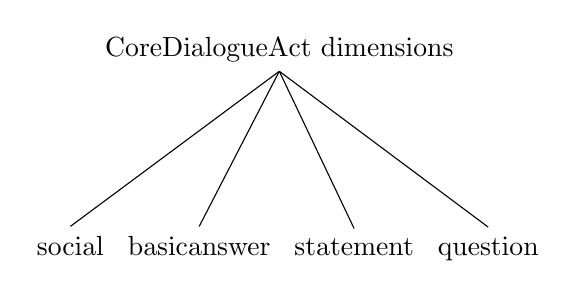
\begin{tikzpicture}
			\tikzset{every tree node/.style={align=center,anchor=base}}
			\tikzset{level 1+/.style={level distance=2\baselineskip}}
			\tikzset{frontier/.style={distance from root=6\baselineskip}}
			\Tree [.{CoreDialogueAct dimensions} social basicanswer statement question ]
		\end{tikzpicture}
	\end{center}
\end{frame}

\begin{frame}[fragile]
\frametitle{Social dimension}
	\begin{center}
		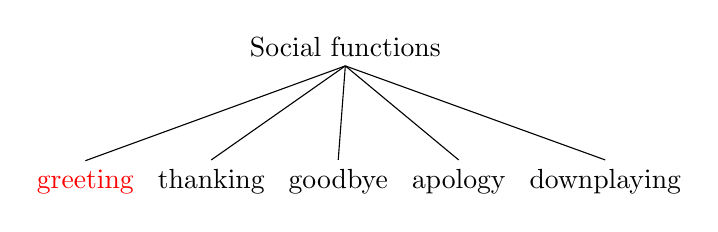
\begin{tikzpicture}
			\tikzset{every tree node/.style={align=center,anchor=base}}
			\tikzset{level 1+/.style={level distance=2\baselineskip}}
			\tikzset{frontier/.style={distance from root=4\baselineskip}}
			\Tree [.{Social functions} \node[color=red]{greeting}; thanking goodbye apology downplaying ]
		\end{tikzpicture}
	\end{center}
	\vspace{15pt}
	\begin{columns}
		\begin{column}{0.65\textwidth}
		{\color{teal} 
			\texttt{U: Good morning.}\\
			\vspace{10pt}
			\texttt{U: Nice to meet you.}\\
			\vspace{10pt}
			\texttt{U: Hello!}\\
		}
		\end{column}
		\begin{column}{0.35\textwidth}
			\footnotesize
			\texttt{CoreDialogueAct:} \\
				\vspace{10pt}
				$\begin{bmatrix}
						\texttt{Dimension:}    & \texttt{social}\\ 
						\texttt{Function:}     & \texttt{greeting}\\ 
				\end{bmatrix}$
		\end{column}
	\end{columns}
\end{frame}

\begin{frame}[fragile]
\frametitle{Social dimension}
	\begin{center}
		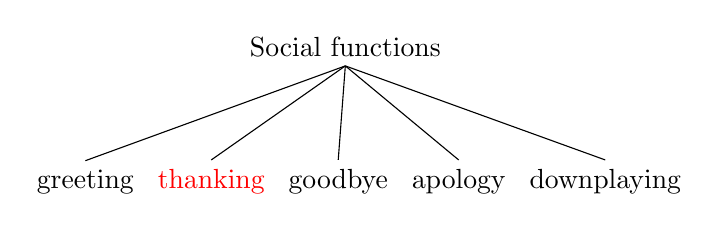
\begin{tikzpicture}
			\tikzset{every tree node/.style={align=center,anchor=base}}
			\tikzset{level 1+/.style={level distance=2\baselineskip}}
			\tikzset{frontier/.style={distance from root=4\baselineskip}}
			\Tree [.{Social functions} greeting \node[color=red]{thanking}; goodbye apology downplaying ]
		\end{tikzpicture}
	\end{center}
	\vspace{15pt}
	\begin{columns}
		\begin{column}{0.65\textwidth}
		{\color{teal} 
			\texttt{U: Thanks!}\\
			\vspace{10pt}
			\texttt{U: Thank you very much.}\\
			\vspace{10pt}
			\texttt{U: I'm so thankful!}\\
		}
		\end{column}
		\begin{column}{0.35\textwidth}
			\footnotesize
			\texttt{CoreDialogueAct:} \\
				\vspace{10pt}
				$\begin{bmatrix}
						\texttt{Dimension:}    & \texttt{social}\\ 
						\texttt{Function:}     & \texttt{thanking}\\ 
				\end{bmatrix}$
		\end{column}
	\end{columns}
\end{frame}

\begin{frame}[fragile]
\frametitle{Social dimension}
	\begin{center}
		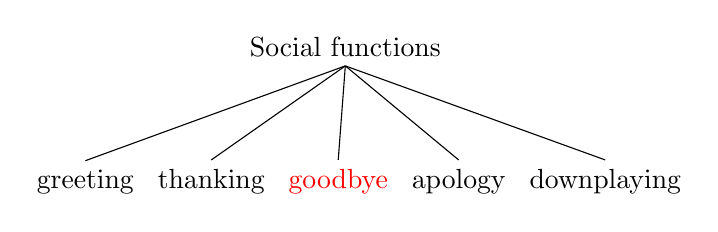
\begin{tikzpicture}
			\tikzset{every tree node/.style={align=center,anchor=base}}
			\tikzset{level 1+/.style={level distance=2\baselineskip}}
			\tikzset{frontier/.style={distance from root=4\baselineskip}}
			\Tree [.{Social functions} greeting thanking \node[color=red]{goodbye}; apology downplaying ]
		\end{tikzpicture}
	\end{center}
	\vspace{15pt}
	\begin{columns}
		\begin{column}{0.65\textwidth}
		{\color{teal} 
			\texttt{U: Have a good day!}\\
			\vspace{10pt}
			\texttt{U: See you later.}\\
			\vspace{10pt}
			\texttt{U: Bye!}\\
		}
		\end{column}
		\begin{column}{0.35\textwidth}
			\footnotesize
			\texttt{CoreDialogueAct:} \\
				\vspace{10pt}
				$\begin{bmatrix}
						\texttt{Dimension:}    & \texttt{social}\\ 
						\texttt{Function:}     & \texttt{goodbye}\\ 
				\end{bmatrix}$
		\end{column}
	\end{columns}
\end{frame}

\begin{frame}[fragile]
\frametitle{Social dimension}
	\begin{center}
		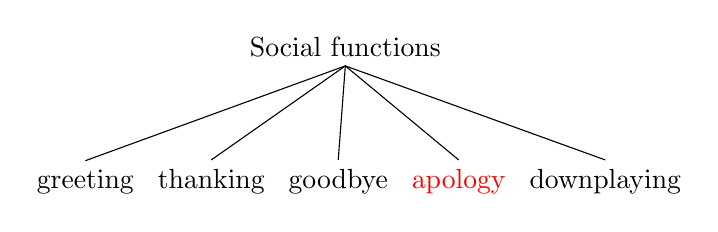
\begin{tikzpicture}
			\tikzset{every tree node/.style={align=center,anchor=base}}
			\tikzset{level 1+/.style={level distance=2\baselineskip}}
			\tikzset{frontier/.style={distance from root=4\baselineskip}}
			\Tree [.{Social functions} greeting thanking goodbye \node[color=red]{apology}; downplaying ]
		\end{tikzpicture}
	\end{center}
	\vspace{15pt}
	\begin{columns}
		\begin{column}{0.65\textwidth}
		{\color{teal} 
			\texttt{U: I'm sorry!}\\
			\vspace{10pt}
			\texttt{U: Excuse me.}\\
			\vspace{10pt}
			\texttt{U: My sincere apologies.}\\
		}
		\end{column}
		\begin{column}{0.35\textwidth}
			\footnotesize
			\texttt{CoreDialogueAct:} \\
				\vspace{10pt}
				$\begin{bmatrix}
						\texttt{Dimension:}    & \texttt{social}\\ 
						\texttt{Function:}     & \texttt{apology}\\ 
				\end{bmatrix}$
		\end{column}
	\end{columns}
\end{frame}


\begin{frame}[fragile]
\frametitle{Social dimension}
	\begin{center}
		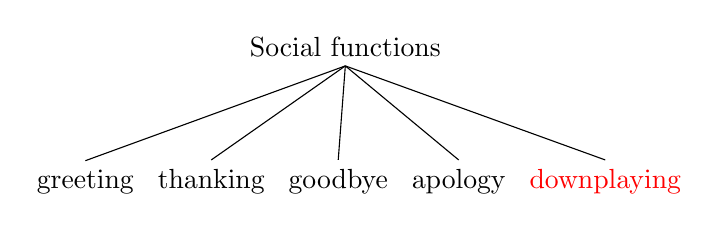
\begin{tikzpicture}
			\tikzset{every tree node/.style={align=center,anchor=base}}
			\tikzset{level 1+/.style={level distance=2\baselineskip}}
			\tikzset{frontier/.style={distance from root=4\baselineskip}}
			\Tree [.{Social functions} greeting thanking goodbye apology \node[color=red]{downplaying}; ]
		\end{tikzpicture}
	\end{center}
	\vspace{15pt}
	\begin{columns}
		\begin{column}{0.60\textwidth}
		{\color{teal} 
			\texttt{U: You're welcome!}\\
			\vspace{10pt}
			\texttt{U: Not at all.}\\
			\vspace{10pt}
			\texttt{U: Don't mention it.}\\
		}
		\end{column}
		\begin{column}{0.40\textwidth}
			\footnotesize
			\texttt{CoreDialogueAct:} \\
				\vspace{10pt}
				$\begin{bmatrix}
						\texttt{Dimension:}    & \texttt{social}\\ 
						\texttt{Function:}     & \texttt{downplaying}\\ 
				\end{bmatrix}$
		\end{column}
	\end{columns}
\end{frame}

\begin{frame}[fragile]
\frametitle{Basicanswer dimension}
	\begin{center}
		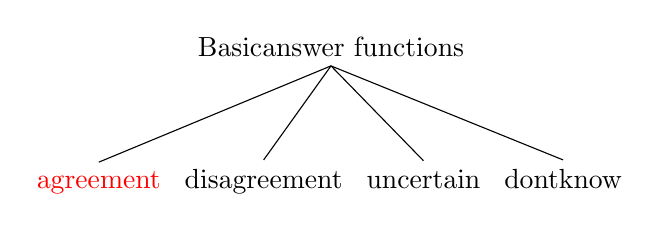
\begin{tikzpicture}
			\tikzset{every tree node/.style={align=center,anchor=base}}
			\tikzset{level 1+/.style={level distance=2\baselineskip}}
			\tikzset{frontier/.style={distance from root=4\baselineskip}}
			\Tree [.{Basicanswer functions} \node[color=red]{agreement}; disagreement uncertain dontknow ]
		\end{tikzpicture}
	\end{center}
	\vspace{15pt}
	\begin{columns}
		\begin{column}{0.60\textwidth}
		{\color{teal} 
			\texttt{U: Yes.}\\
			\vspace{10pt}
			\texttt{U: Ok.}\\
			\vspace{10pt}
			\texttt{U: That's right.}\\
		}
		\end{column}
		\begin{column}{0.40\textwidth}
			\footnotesize
			\texttt{CoreDialogueAct:} \\
				\vspace{10pt}
				$\begin{bmatrix}
						\texttt{Dimension:}    & \texttt{basicanswer}\\ 
						\texttt{Function:}     & \texttt{agreement}\\ 
				\end{bmatrix}$
		\end{column}
	\end{columns}
\end{frame}

\begin{frame}[fragile]
\frametitle{Basicanswer dimension}
	\begin{center}
		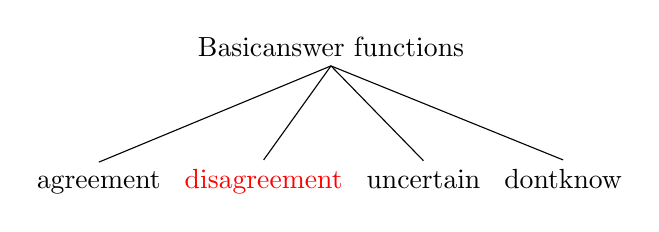
\begin{tikzpicture}
			\tikzset{every tree node/.style={align=center,anchor=base}}
			\tikzset{level 1+/.style={level distance=2\baselineskip}}
			\tikzset{frontier/.style={distance from root=4\baselineskip}}
			\Tree [.{Basicanswer functions} agreement \node[color=red]{disagreement}; uncertain dontknow ]
		\end{tikzpicture}
	\end{center}
	\vspace{15pt}
	\begin{columns}
		\begin{column}{0.58\textwidth}
		{\color{teal} 
			\texttt{U: No.}\\
			\vspace{10pt}
			\texttt{U: No way.}\\
			\vspace{10pt}
			\texttt{U: I can't agree.}\\
		}
		\end{column}
		\begin{column}{0.42\textwidth}
			\footnotesize
			\texttt{CoreDialogueAct:} \\
				\vspace{10pt}
				$\begin{bmatrix}
						\texttt{Dimension:}    & \texttt{basicanswer}\\ 
						\texttt{Function:}     & \texttt{disagreement}\\ 
				\end{bmatrix}$
		\end{column}
	\end{columns}
\end{frame}

\begin{frame}[fragile]
\frametitle{Basicanswer dimension}
	\begin{center}
		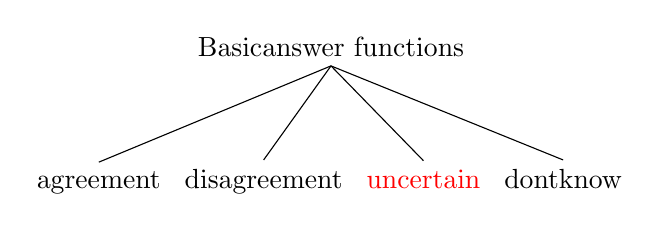
\begin{tikzpicture}
			\tikzset{every tree node/.style={align=center,anchor=base}}
			\tikzset{level 1+/.style={level distance=2\baselineskip}}
			\tikzset{frontier/.style={distance from root=4\baselineskip}}
			\Tree [.{Basicanswer functions} agreement disagreement \node[color=red]{uncertain}; dontknow ]
		\end{tikzpicture}
	\end{center}
	\vspace{15pt}
	\begin{columns}
		\begin{column}{0.60\textwidth}
		{\color{teal} 
			\texttt{U: Maybe.}\\
			\vspace{10pt}
			\texttt{U: Perhaps.}\\
			\vspace{10pt}
			\texttt{U: Probably.}\\
		}
		\end{column}
		\begin{column}{0.40\textwidth}
			\footnotesize
			\texttt{CoreDialogueAct:} \\
				\vspace{10pt}
				$\begin{bmatrix}
						\texttt{Dimension:}    & \texttt{basicanswer}\\ 
						\texttt{Function:}     & \texttt{uncertain}\\ 
				\end{bmatrix}$
		\end{column}
	\end{columns}
\end{frame}

\begin{frame}[fragile]
\frametitle{Basicanswer dimension}
	\begin{center}
		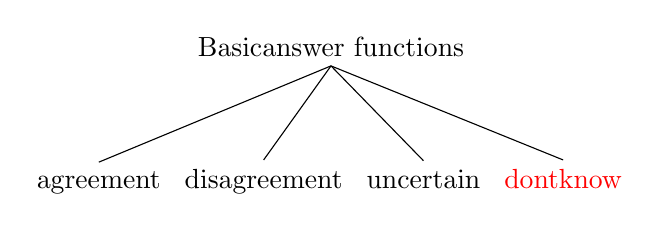
\begin{tikzpicture}
			\tikzset{every tree node/.style={align=center,anchor=base}}
			\tikzset{level 1+/.style={level distance=2\baselineskip}}
			\tikzset{frontier/.style={distance from root=4\baselineskip}}
			\Tree [.{Basicanswer functions} agreement disagreement uncertain \node[color=red]{dontknow}; ]
		\end{tikzpicture}
	\end{center}
	\vspace{15pt}
	\begin{columns}
		\begin{column}{0.60\textwidth}
		{\color{teal} 
			\texttt{U: I don't know.}\\
			\vspace{10pt}
			\texttt{U: I don't remember.}\\
			\vspace{10pt}
			\texttt{U: I have no idea.}\\
		}
		\end{column}
		\begin{column}{0.40\textwidth}
			\footnotesize
			\texttt{CoreDialogueAct:} \\
				\vspace{10pt}
				$\begin{bmatrix}
						\texttt{Dimension:}    & \texttt{basicanswer}\\ 
						\texttt{Function:}     & \texttt{dontknow}\\ 
				\end{bmatrix}$
		\end{column}
	\end{columns}
\end{frame}

\begin{frame}[fragile]
\frametitle{Statement dimension}
	\begin{center}
		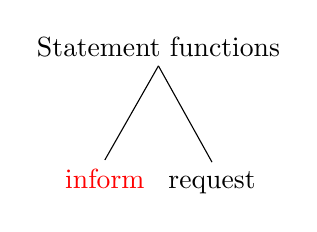
\begin{tikzpicture}
			\tikzset{every tree node/.style={align=center,anchor=base}}
			\tikzset{level 1+/.style={level distance=2\baselineskip}}
			\tikzset{frontier/.style={distance from root=4\baselineskip}}
			\Tree [.{Statement functions} \node[color=red]{inform}; request ]
		\end{tikzpicture}
	\end{center}
	\vspace{15pt}
	\begin{columns}
		\begin{column}{0.60\textwidth}
		{\color{teal} 
			\texttt{U: My name is ...}\\
			\vspace{10pt}
			\texttt{U: I live in ...}\\
			\vspace{10pt}
			\texttt{U: I don't want nothing else.}\\
		}
		\end{column}
		\begin{column}{0.40\textwidth}
			\footnotesize
			\texttt{CoreDialogueAct:} \\
				\vspace{10pt}
				$\begin{bmatrix}
						\texttt{Dimension:}    & \texttt{statement}\\ 
						\texttt{Function:}     & \texttt{inform}\\ 
				\end{bmatrix}$
		\end{column}
	\end{columns}
\end{frame}

\begin{frame}[fragile]
\frametitle{Statement dimension}
	\begin{center}
		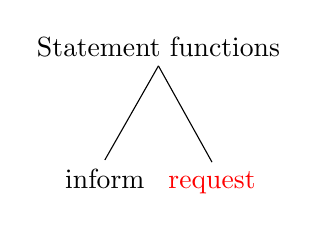
\begin{tikzpicture}
			\tikzset{every tree node/.style={align=center,anchor=base}}
			\tikzset{level 1+/.style={level distance=2\baselineskip}}
			\tikzset{frontier/.style={distance from root=4\baselineskip}}
			\Tree [.{Statement functions} inform \node[color=red]{request}; ]
		\end{tikzpicture}
	\end{center}
	\vspace{15pt}
	\begin{columns}
		\begin{column}{0.60\textwidth}
		{\color{teal} 
			\texttt{U: I want ...}\\
			\vspace{10pt}
			\texttt{U: I would need ...}\\
			\vspace{10pt}
			\texttt{U: Would you mind if ...?}\\
		}
		\end{column}
		\begin{column}{0.40\textwidth}
			\footnotesize
			\texttt{CoreDialogueAct:} \\
				\vspace{10pt}
				$\begin{bmatrix}
						\texttt{Dimension:}    & \texttt{statement}\\ 
						\texttt{Function:}     & \texttt{request}\\ 
				\end{bmatrix}$
		\end{column}
	\end{columns}
\end{frame}

\begin{frame}[fragile]
\frametitle{Question dimension}
	\begin{center}
		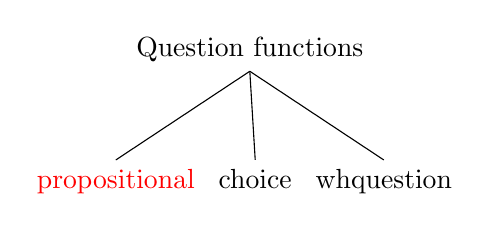
\begin{tikzpicture}
			\tikzset{every tree node/.style={align=center,anchor=base}}
			\tikzset{level 1+/.style={level distance=2\baselineskip}}
			\tikzset{frontier/.style={distance from root=4\baselineskip}}
			\Tree [.{Question functions} \node[color=red]{propositional}; choice whquestion ]
		\end{tikzpicture}
	\end{center}
	\vspace{15pt}
	\begin{columns}
		\begin{column}{0.58\textwidth}
		{\color{red} 
			\texttt{S: Do you agree with the date of the appointment?}\\}
			\vspace{10pt}
		{\color{teal} 
			\texttt{U: Do you like basketball?}\\
			\vspace{10pt}
			\texttt{U: Do you I am right?}\\
		}
		\end{column}
		\begin{column}{0.42\textwidth}
			\footnotesize
			\texttt{CoreDialogueAct:} \\
				\vspace{10pt}
				$\begin{bmatrix}
						\texttt{Dimension:}    & \texttt{question}\\ 
						\texttt{Function:}     & \texttt{propositional}\\ 
				\end{bmatrix}$
		\end{column}
	\end{columns}
\end{frame}

\begin{frame}[fragile]
\frametitle{Question dimension}
	\begin{center}
		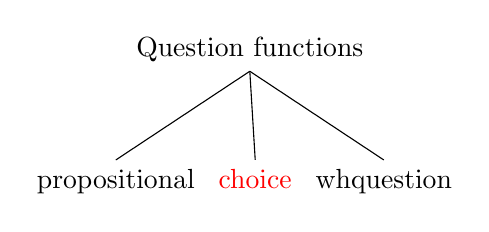
\begin{tikzpicture}
			\tikzset{every tree node/.style={align=center,anchor=base}}
			\tikzset{level 1+/.style={level distance=2\baselineskip}}
			\tikzset{frontier/.style={distance from root=4\baselineskip}}
			\Tree [.{Question functions} propositional \node[color=red]{choice}; whquestion ]
		\end{tikzpicture}
	\end{center}
	\vspace{15pt}
	\begin{columns}
		\begin{column}{0.60\textwidth}
		\small
		{\color{red} 
			\texttt{S: What do you want to do first, make a bank transfer or locate the nearest ATM?}\\
			\vspace{10pt}
			\texttt{S: Do you prefer coffee or tea?}\\
			\vspace{10pt}
			\texttt{S: When do you want the appointment, in the morning or in the afternoon?}\\
		}
		\end{column}
		\begin{column}{0.40\textwidth}
			\footnotesize
			\texttt{CoreDialogueAct:} \\
				\vspace{10pt}
				$\begin{bmatrix}
						\texttt{Dimension:}    & \texttt{question}\\ 
						\texttt{Function:}     & \texttt{choice}\\ 
				\end{bmatrix}$
		\end{column}
	\end{columns}
\end{frame}

\begin{frame}[fragile]
\frametitle{Question dimension}
	\begin{center}
		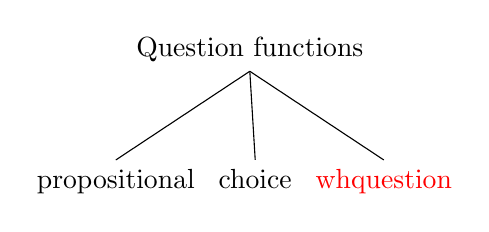
\begin{tikzpicture}
			\tikzset{every tree node/.style={align=center,anchor=base}}
			\tikzset{level 1+/.style={level distance=2\baselineskip}}
			\tikzset{frontier/.style={distance from root=4\baselineskip}}
			\Tree [.{Question functions} propositional choice \node[color=red]{whquestion}; ]
		\end{tikzpicture}
	\end{center}
	\vspace{15pt}
	\begin{columns}
		\begin{column}{0.60\textwidth}
		{\color{teal} 
			\texttt{U: What time is it?}\\
			\vspace{10pt}
			\texttt{U: How much is the doctor appointment?}\\
			\vspace{10pt}
			\texttt{U: Where is the nearest ATM?}\\
		}
		\end{column}
		\begin{column}{0.40\textwidth}
			\footnotesize
			\texttt{CoreDialogueAct:} \\
				\vspace{10pt}
				$\begin{bmatrix}
						\texttt{Dimension:}    & \texttt{question}\\ 
						\texttt{Function:}     & \texttt{whquestion}\\ 
				\end{bmatrix}$
		\end{column}
	\end{columns}
\end{frame}

\begin{frame}[fragile]
\frametitle{\texttt{TaskDialogueAct} structure}
	\begin{itemize}
		\item Dialogue act annotation is used to know the communicative function of user proferences.
		\item This doesn't depend on domain.
		\item But it lacks of semantic information. For example: In \texttt{statement-request} pair we wish to know what user wants to do and the object of his desire.
		\item This kind of information may depend on domain.
	\end{itemize}
	\scriptsize
	\pause
	\begin{lstlisting}[language=lekta]
classDef:StructureComplex ( 
	TaskDialogueAct : ( Action, Scope ) )

classDef:StructureBatch (	Action : ( ActionDomain ) )

classDef:ElementLiteral (	ActionDomain )
classDef:ElementLiteral (	Scope )
	\end{lstlisting}	
\end{frame}

\begin{frame}[fragile]
\frametitle{Domains implemented}
So we have implemented a couple of domains to do some testings:
	\setbeamercolor{block title}{use=structure,fg=white,bg=green!75!black}
	\setbeamercolor{block body}{use=structure,fg=black,bg=green!10!white}
	\begin{block}{Medical appointment}
		\begin{itemize}
			\item Task 1: \texttt{ActionDomain = `book'. Scope = `appointment'}
		\end{itemize}	
	\end{block}
	\pause
	\setbeamercolor{block title}{use=structure,fg=white,bg=green!75!black}
	\setbeamercolor{block body}{use=structure,fg=black,bg=green!10!white}
	\begin{block}{Banking management}
		\begin{itemize}
			\item Task 1: \texttt{ActionDomain = `consult'. Scope = `bankaccount'}
			\item Task 2: \texttt{ActionDomain = `locate'. Scope = `atm'}
			\item Task 3: \texttt{ActionDomain = `execute'. Scope = `transfer'}
		\end{itemize}
	\end{block}
\end{frame}

\begin{frame}[fragile]
\frametitle{Verb lemmas}
To detect actions in understanding stage, we associate some verbs lemmas to a certain action:
	\footnotesize
	\setbeamercolor{block title}{use=structure,fg=white,bg=green!75!black}
	\setbeamercolor{block body}{use=structure,fg=black,bg=green!10!white}
	\begin{block}{ActionDomain = `book'}
		book, establish, have, \textbf{make}, get, schedule, ask, set up, ...\\
		\vspace{10pt}
		{\color{teal} 
			\texttt{U: I want to get an appointment.}\\
			\texttt{U: I would like to make medical appointment.}\\
		}
	\end{block}
	\pause
	\footnotesize
	\setbeamercolor{block title}{use=structure,fg=white,bg=green!75!black}
	\setbeamercolor{block body}{use=structure,fg=black,bg=green!10!white}
	\begin{block}{ActionDomain = `execute'}
		\textbf{make}, move, execute, perform, do, accomplish, fulfill, effectuate, carry out, complete, ...\\
		\vspace{10pt}
		{\color{teal} 
			\texttt{U: I want to perform a bank transfer.}\\
			\texttt{U: I would like to make a transfer.}\\
		}
	\end{block}
	\pause
	Please note that a verb lemma can be associated with more than one \texttt{ActionDomain} (ambiguities everywhere!).
\end{frame}

\begin{frame}[fragile]
\frametitle{Parameters}
A `parameter' is some kind of useful information to complete a task. For example a \texttt{`datetime'} or an \texttt{`accountnumber'}.
\scriptsize
\begin{lstlisting}[language=lekta]
classDef:StructureComplex
(
	Parameter :
	(
		ParameterCategory, // 'terminal', 'and', 'or', ...
		ParameterType,     // 'datetime', 'accountnumber', ...
		ParameterValue,    // Similar to math expressions
		ParameterOperand1, 
		ParameterOperand2
	)
)
\end{lstlisting}
\pause
	\setbeamercolor{block title}{use=structure,fg=white,bg=green!75!black}
	\setbeamercolor{block body}{use=structure,fg=black,bg=green!10!white}
	\begin{block}{Example of \texttt{ParameterCategory}}
		{\color{teal} 
			\texttt{U: I want an appointment for tomorrow or the day after tomorrow.}\\
			\vspace{10pt}
			\texttt{U: My telephone numbers are 1234 and 5678.}\\
		}
	\end{block}
\end{frame}

\begin{frame}[fragile]
\frametitle{Parameters}
This information is provided by the user and may be compulsory ({\color{red}red}) or optative ({\color{teal}green})
	\scriptsize
	\setbeamercolor{block title}{use=structure,fg=white,bg=green!75!black}
	\setbeamercolor{block body}{use=structure,fg=black,bg=green!10!white}
	\begin{block}{Examples}
		\begin{itemize}
			\item \texttt{BookAppointment} task:
			\begin{itemize}
				\item \scriptsize{\color{red} \texttt{medicalspeciality}}
				\item \scriptsize{\color{red} \texttt{countryplace}}
				\item \scriptsize{\color{red} \texttt{phonenumber}}
				\item \scriptsize{\color{red} \texttt{peselnumber}} (Ok, it's a polish medical appointment!)
				\item \scriptsize{\color{teal} \texttt{datetime}}
			\end{itemize}
			\item \texttt{ConsultBankaccount} task: 
			\begin{itemize}
				\item \scriptsize{\color{red} \texttt{accountnumber}}
			\end{itemize}
			\item \texttt{LocateAtm} task: 
			\begin{itemize}
				\item \scriptsize{\color{red} \texttt{countryplace}}
			\end{itemize}
			\item \texttt{ExecuteTransfer} task: 
			\begin{itemize}
				\item \scriptsize{\color{red} \texttt{accountnumber}}
				\item \scriptsize{\color{red} \texttt{moneyamount}}
			\end{itemize}
		\end{itemize}
	\end{block}
\end{frame}

\begin{frame}[fragile]
\frametitle{Parameters classification}
\begin{itemize}
	\item Parameteres can be classified depending upon its domain. 
	\item If it's domain-independent we say that the parameter belongs to ``kernel'' domain.
	\item But take into account that we can move a parameter from its domain to kernel domain in order to make it \textbf{reusable}.
\end{itemize}
	\pause
	\setbeamercolor{block title}{use=structure,fg=white,bg=green!75!black}
	\setbeamercolor{block body}{use=structure,fg=black,bg=green!10!white}
	\begin{block}{Kernel domain implemented parameters}
	\begin{columns}
		\begin{column}{0.50\textwidth}
			\begin{itemize}
				\item \texttt{countryplace}
				\item \texttt{datetime}
				\item \texttt{letter}
				\item \texttt{moneyamount}
			\end{itemize}
		\end{column}
		\begin{column}{0.50\textwidth}
			\begin{itemize}
				\item \texttt{number}
				\item \texttt{ordinal}
				\item \texttt{phonenumber}
				\item \texttt{signchunk}
			\end{itemize}
		\end{column}
	\end{columns}
	\end{block}
\end{frame}
	
\begin{frame}[fragile]
\frametitle{Parameters classification}
	\setbeamercolor{block title}{use=structure,fg=white,bg=green!75!black}
	\setbeamercolor{block body}{use=structure,fg=black,bg=green!10!white}
	\begin{block}{Medical appointment domain implemented parameters}
		\begin{itemize}
			\item \texttt{medicalspeciality}
			\item \texttt{peselnumber}
		\end{itemize}
	\end{block}
	\setbeamercolor{block title}{use=structure,fg=white,bg=green!75!black}
	\setbeamercolor{block body}{use=structure,fg=black,bg=green!10!white}
	\begin{block}{Banking management domain implemented parameters}
		\begin{itemize}
			\item \texttt{accountnumber}
		\end{itemize}
	\end{block}
\end{frame}
	
\begin{frame}[fragile]
\frametitle{Parameters example: \texttt{datetime}}
\scriptsize
\begin{lstlisting}[language=lekta]
classDef:StructureComplex (
		DateTime: (
		BaseDate,
		OffsetDate,
		MinDate,
		MaxDate,
		GeneralTime
	)
)

classDef:StructureComplex (
		GeneralTime: (
		BaseTime,
		OffsetTime,
		MinTime,
		MaxTime
	)
)
\end{lstlisting}
\end{frame}
	
\begin{frame}[fragile]
\frametitle{Parameters example: \texttt{datetime}}
{\color{teal} 
	\texttt{U: Starting next thursday until 3pm to the day after 25 of august from noon to a quarter to nine in the afternoon.}\\
}
\pause
\vspace{15pt}
\scriptsize
\begin{lstlisting}[language=lekta]
(DateTime:
   (MinDate:(GeneralTime:(MaxTime:(BaseTime:(Hour:15))),
             OffsetDate :(DirectionOfTime:'forward',
                          Date           :(DayInWeek:4),
                          DayInWeekOffset:1)),
    MaxDate:(GeneralTime:(MinTime:(BaseTime:(Hour:12)),
                          MaxTime:(BaseTime:(Hour:20,
                                             Minute:45))),
             OffsetDate :(DirectionOfTime:'forward',
                          Date           :(Day:1)),
             BaseDate   :(Day  :25,
                          Month:8))))))
\end{lstlisting}
\end{frame}
	
\begin{frame}[fragile]
\frametitle{Parameters example: \texttt{countryplace}}
\scriptsize
\begin{lstlisting}[language=lekta]
classDef:StructureComplex ( 
		CountryPlace : (
		CountryName,
		CountryZone,
		CountryRegion,
		CountryProvince,
		CountryTown
	)
)

classDef:ElementLiteral (
	CountryName,
	CountryZone,
	CountryRegion,
	CountryProvince,
	CountryTown
)
\end{lstlisting}
\end{frame}

\begin{frame}[fragile]
\frametitle{Parameters example: \texttt{countryplace}}
{\small
\begin{itemize}
	\item We have used \textbf{NUTS} (Nomenclature of Territorial Units for Statistics) and \textbf{LAU} (Local Administrative Unit), two standards developed by European Union.
	\item We have, in the lexicon, all cities and towns of countries belonging to EU (except UK whose format file is different as usual!).
	\item This lexicon is expressed in the local language so we have Sevilla, but not Seville. We have Warszawa but not Warsaw.
\end{itemize}}
	\pause
	\scriptsize
	\setbeamercolor{block title}{use=structure,fg=white,bg=green!75!black}
	\setbeamercolor{block body}{use=structure,fg=black,bg=green!10!white}
	\begin{block}{Some examples}
	\begin{itemize}
		\item France: 39096 entries.
		\item Germany: 11167 entries.
		\item Bulgary: 10532 entries.
		\item Spain: 8837 entries.
		\item Italy: 8161 entries.
		\item Poland: 2478 entries. 
	\end{itemize}
	\end{block}
\end{frame}
	
\begin{frame}[fragile]
\frametitle{\texttt{DialogueAct} structure}
So we define this dialogue act type in Fluency:
\scriptsize
\begin{lstlisting}[language=lekta]
classDef:StructureComplex 
( 
 	DialogueAct :
  	(
		CoreDialogueAct,
		TaskDialogueAct,
		Parameters
	)
)	

classDef:StructureBatch
(
	Parameters :
	(
		Parameter
	)
)
\end{lstlisting}
\end{frame}
	

\begin{frame}[fragile]
\frametitle{Dialogue act annotation full example}
{\color{teal} 
	\texttt{U: I want to book an appointment for tomorrow to the dentist.}\\
}
\pause
\vspace{15pt}
\tiny
\begin{lstlisting}[language=lekta]
(DialogueAct:
   (CoreDialogueAct:(Dimension:'statement',
                     Function :'request')),
   (TaskDialogueAct:(Action:{(ActionDomain:'book')}
                     Scope:'appointment')),
   (Parameters:     {(Parameter:
                      (ParameterValue:
                       (DateTime:(OffsetDate:(DirectionOfTime:'forward',
                                              Date           :(Day:1))))),
                       ParameterCategory:'terminal',
                       ParameterType    :'datetime'),
                     (Parameter:
                      (ParameterValue:
                       (MedicalSpeciality:(SpecialityName:'Orthodontics'),
                       ParameterCategory:'terminal',
                       ParameterType    :'medicalspeciality')})
\end{lstlisting}
\end{frame}
				
\subsection{Fluency dialogue manager}

\begin{frame}
\frametitle{Script model}
\begin{itemize}
	\item Every task in all domains are modelled like scripts.
	\item A script consist of four parts:
	\begin{itemize}
	  \item \textbf{Descriptor:} Literal identificator to distingush this script among others.
		\item \textbf{Trigger:} Information that user must provide in order to activate the script.
		\item \textbf{InfoItems:} Place where the information is stored when script is activated. Can be provided by the user or the system itself.
		\item \textbf{Phases:} Subtasks needed to be performed in order to execute bigger one.
			\begin{itemize}
				\item Every phase has a priority level (0 the highest priority).
				\item Election mode: If all phases of level \emph{n} are finished we select a \emph{n+1} level phase randomly. 
			\end{itemize}
	\end{itemize}
	\item All scripts and states are stored in mindboard structures.
\end{itemize}
\end{frame}

\begin{frame}[fragile]
\frametitle{Script model: \texttt{ConsultBalance} script}
\scriptsize
\begin{lstlisting}[language=lekta]
Descriptor: 'ConsultBalance'

Trigger.CoreDialogueAct: ('statement', 'request')
Trigger.ActionDomain: 'consult' 
Trigger.Scope: 'bankaccount'
Trigger.Parameter: 'accountnumber'			
			
InfoItem.Parameter1: 'accountnumber' // Provided by the user
InfoItem.Parameter2: 'moneyamount' // Provided by the system
\end{lstlisting}

\tikzstyle{VertexStyle} = [shape            = rectangle,
                           minimum width    = 6ex,%
                           draw]
\tikzstyle{EdgeStyle}   = [->,>=stealth']      
\begin{center}
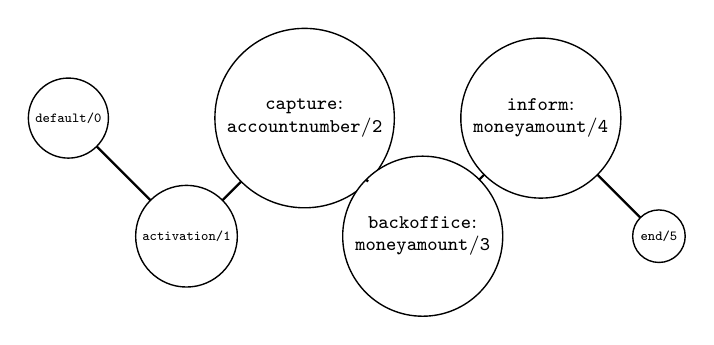
\begin{tikzpicture}[scale=1.0] 
	\SetGraphUnit{1.5} 
	\Vertex[L=\tiny\texttt{default/0}]{0} 	
		  \SOEA[L=\tiny\texttt{activation/1}](0){1}
			\NOEA[L=$\genfrac{}{}{0pt}{1}{\mathtt{capture:}}{\mathtt{accountnumber/2}}$](1){2}
			\SOEA[L=$\genfrac{}{}{0pt}{1}{\mathtt{backoffice:}}{\mathtt{moneyamount/3}}$](2){3}
			\NOEA[L=$\genfrac{}{}{0pt}{1}{\mathtt{inform:}}{\mathtt{moneyamount/4}}$](3){4}
      \SOEA[L=\tiny\texttt{end/5}](4){5}
  \Edges(0,1,2,3,4,5)
\end{tikzpicture}
\end{center}
\end{frame}

\begin{frame}[fragile]
\frametitle{Script model: \texttt{LocateAtm} script}
\scriptsize
\begin{lstlisting}[language=lekta]
Descriptor: 'LocateAtm'

Trigger.CoreDialogueAct: ('statement', 'request')
Trigger.ActionDomain: 'locate' 
Trigger.Scope: 'atm'
Trigger.Parameter: 'countryplace'			
			
InfoItem.Parameter1: 'countryplace' // Provided by the user
InfoItem.Parameter2: 'localization' // Provided by the system
\end{lstlisting}

\tikzstyle{VertexStyle} = [shape            = rectangle,
                           minimum width    = 6ex,%
                           draw]
\tikzstyle{EdgeStyle}   = [->,>=stealth']      
\begin{center}
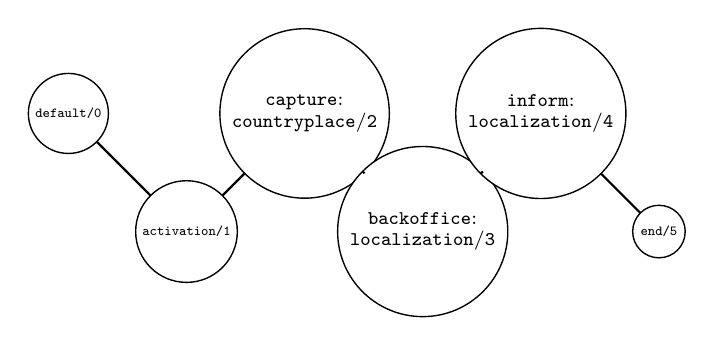
\begin{tikzpicture}[scale=1.0] 
	\SetGraphUnit{1.5} 
	\Vertex[L=\tiny\texttt{default/0}]{0} 	
		  \SOEA[L=\tiny\texttt{activation/1}](0){1}
			\NOEA[L=$\genfrac{}{}{0pt}{1}{\mathtt{capture:}}{\mathtt{countryplace/2}}$](1){2}
			\SOEA[L=$\genfrac{}{}{0pt}{1}{\mathtt{backoffice:}}{\mathtt{localization/3}}$](2){3}
			\NOEA[L=$\genfrac{}{}{0pt}{1}{\mathtt{inform:}}{\mathtt{localization/4}}$](3){4}
      \SOEA[L=\tiny\texttt{end/5}](4){5}
  \Edges(0,1,2,3,4,5)
\end{tikzpicture}
\end{center}
\end{frame}

\begin{frame}[fragile]
\frametitle{Script model: \texttt{MakeTransfer} script}
\scriptsize
\begin{lstlisting}[language=lekta]
Descriptor: 'MakeTransfer'

Trigger.CoreDialogueAct: ('statement', 'request')
Trigger.ActionDomain: 'execute' 
Trigger.Scope: 'transfer'
Trigger.Parameter1: 'accountnumber'			
Trigger.Parameter2: 'moneyamount'			
			
InfoItem.Parameter1: 'accountnumber' // Provided by the user
InfoItem.Parameter2: 'moneyamount'   // Provided by the user
\end{lstlisting}

\tikzstyle{VertexStyle} = [shape            = rectangle,
                           minimum width    = 6ex,%
                           draw]
\tikzstyle{EdgeStyle}   = [->,>=stealth']      
\begin{center}
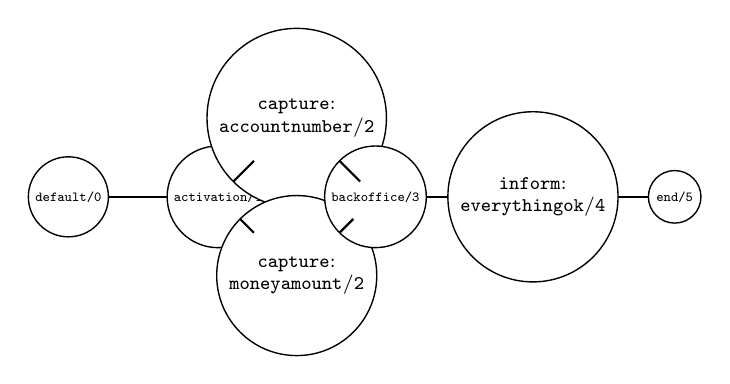
\begin{tikzpicture}[scale=1.0] 
	\SetGraphUnit{1.9} 
	\Vertex[L=\tiny\texttt{default/0}]{0} 	
		  \EA[L=\tiny\texttt{activation/1}](0){1}
			\SetGraphUnit{1} 
			\NOEA[L=$\genfrac{}{}{0pt}{1}{\mathtt{capture:}}{\mathtt{accountnumber/2}}$](1){2}
			\SOEA[L=$\genfrac{}{}{0pt}{1}{\mathtt{capture:}}{\mathtt{moneyamount/2}}$](1){6}
			\SOEA[L=\tiny\texttt{backoffice/3}](2){3}
			\SetGraphUnit{2.0} 
			\EA[L=$\genfrac{}{}{0pt}{1}{\mathtt{inform:}}{\mathtt{everythingok/4}}$](3){4}
			\SetGraphUnit{1.8} 
      \EA[L=\tiny\texttt{end/5}](4){5}
  \Edges(0,1,2,3,4,5)
	\Edges(1,6,3)
\end{tikzpicture}
\end{center}
\end{frame}


\begin{frame}[fragile]
\frametitle{Script model: \texttt{BookAppointment} script}
\scriptsize
\begin{lstlisting}[language=lekta]
Descriptor: 'BookAppointment'

Trigger.CoreDialogueAct: ('statement', 'request')
Trigger.ActionDomain: 'book' 
Trigger.Scope: 'appointment'
Trigger.Parameter1: 'medicalspeciality'			
Trigger.Parameter2: 'countryplace'			
Trigger.Parameter3: 'datetime'			
Trigger.Parameter4: 'phonenumber'			
Trigger.Parameter5: 'peselnumber'			

InfoItem.Parameter1: 'medicalspeciality' 
InfoItem.Parameter2: 'countryplace'      
InfoItem.Parameter3: 'datetime'          
InfoItem.Parameter4: 'phonenumber'       
InfoItem.Parameter5: 'peselnumber'       
\end{lstlisting}
\end{frame}

\begin{frame}[fragile]
\frametitle{Script model: \texttt{BookAppointment} script}
\scriptsize
\tikzstyle{VertexStyle} = [shape            = rectangle,
                           minimum width    = 6ex,%
                           draw]
\tikzstyle{EdgeStyle}   = [->,>=stealth']      
\begin{center}
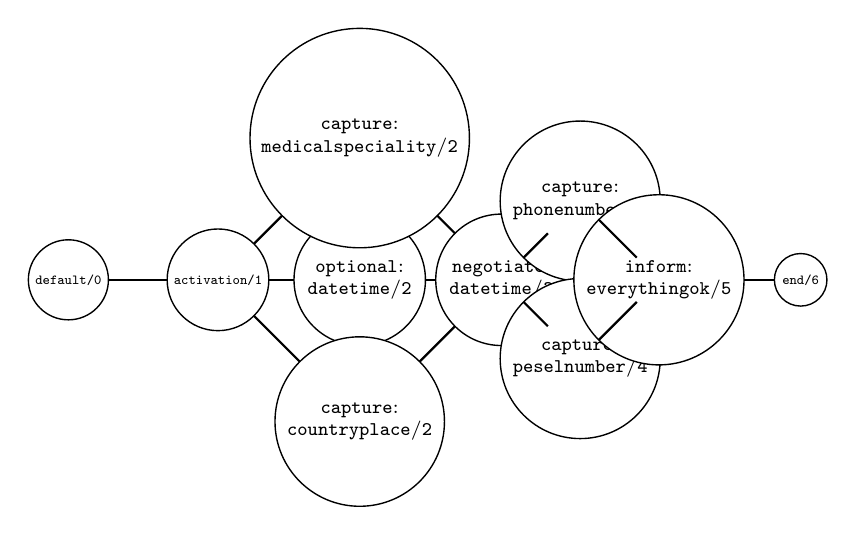
\begin{tikzpicture}[scale=1.0] 
	\SetGraphUnit{1.9} 
	\Vertex[L=\tiny\texttt{default/0}]{0} 	
		  \EA[L=\tiny\texttt{activation/1}](0){1}
			\SetGraphUnit{1.8} 
			\EA[L=$\genfrac{}{}{0pt}{1}{\mathtt{optional:}}{\mathtt{datetime/2}}$](1){2}
			\NOEA[L=$\genfrac{}{}{0pt}{1}{\mathtt{capture:}}{\mathtt{medicalspeciality/2}}$](1){3}
			\SOEA[L=$\genfrac{}{}{0pt}{1}{\mathtt{capture:}}{\mathtt{countryplace/2}}$](1){4}
			\EA[L=$\genfrac{}{}{0pt}{1}{\mathtt{negotiate:}}{\mathtt{datetime/3}}$](2){5}
			\SetGraphUnit{1.0} 
			\NOEA[L=$\genfrac{}{}{0pt}{1}{\mathtt{capture:}}{\mathtt{phonenumber/4}}$](5){6}
			\SOEA[L=$\genfrac{}{}{0pt}{1}{\mathtt{capture:}}{\mathtt{peselnumber/4}}$](5){7}
			\SOEA[L=$\genfrac{}{}{0pt}{1}{\mathtt{inform:}}{\mathtt{everythingok/5}}$](6){8}
			\SetGraphUnit{1.8} 
			\EA[L=\tiny\texttt{end/6}](8){9}
  \Edges(0,1,2,5,6)
	\Edges(1,3,5)
	\Edges(1,4,5)
	\Edges(5,7,8,9)
	\Edges(6,8)
\end{tikzpicture}
\end{center}
\end{frame}

\begin{frame}[fragile]
\frametitle{Fluency DM phases}
Every dialogue system turn execute this loop until last phase is reached:
\begin{enumerate}
	\item Start talking.
	\item Digest expectatives.
	\item Digest search scripts.
	\item Activate scripts.
	\item Select current script.
	\item Review states.
	\item Select current node.
	\item Process talking.
	\begin{enumerate}
		\item Execute node (go to 5).
		\item Wait node (go to 9).
	\end{enumerate}
	\item Close talking (go to 1 after user turn).
\end{enumerate}
\end{frame}

\begin{frame}[fragile]
\frametitle{Fluency DM phases}
	\setbeamercolor{block title}{use=structure,fg=white,bg=red!75!black}
	\setbeamercolor{block body}{use=structure,fg=black,bg=red!10!white}
	\begin{block}{1. Start talking}
	\begin{itemize}
		\item Erase output mindboard structures.
	\end{itemize}
	\end{block}
	\pause
	\setbeamercolor{block title}{use=structure,fg=white,bg=red!75!black}
	\setbeamercolor{block body}{use=structure,fg=black,bg=red!10!white}
	\begin{block}{2. Digest expectatives}
	\begin{itemize}
		\item Here we convert some parameters to the types of expected parameters.
		\item For example, if we are expecting a phone number and user says a number, we can transform on into the other.
	\end{itemize}
	\end{block}
	\pause
	\setbeamercolor{block title}{use=structure,fg=white,bg=red!75!black}
	\setbeamercolor{block body}{use=structure,fg=black,bg=red!10!white}
	\begin{block}{3. Digest search scripts}
	\begin{itemize}
		\item We analyze user proferences and create some triggering schemes.
		\item We give a scoring to every scheme to see its relevance.
	\end{itemize}
	\end{block}
\end{frame}

\begin{frame}[fragile]
\frametitle{Fluency DM phases}
	\footnotesize
	\setbeamercolor{block title}{use=structure,fg=white,bg=red!75!black}
	\setbeamercolor{block body}{use=structure,fg=black,bg=red!10!white}
	\begin{block}{4. Activate scripts}
	\begin{itemize}
		\item Depending on triggering schemes from previous phase we select what scripts must be activated.
		\item This is not trivial:
		\begin{itemize}
			\item What happens if comes a parameter from an active script, but not the current?
			\item What happens if comes a parameter from a non-active script?
			\item What happens if we have several triggered scripts with the same scoring?
		\end{itemize}
	\end{itemize}
	\end{block}
	\pause
	\footnotesize
	\setbeamercolor{block title}{use=structure,fg=white,bg=red!75!black}
	\setbeamercolor{block body}{use=structure,fg=black,bg=red!10!white}
	\begin{block}{5. Select current script}
	\begin{itemize}
		\item Previous phase ends sorting the activated scripts stack so we select, as current script, the one placed in the top of the stack.
		\item If we have a recently activated script it's the moment to recover some mid-term memory slots.
	\end{itemize}
	\end{block}
\end{frame}

\begin{frame}[fragile]
\frametitle{Fluency DM phases}
	\setbeamercolor{block title}{use=structure,fg=white,bg=red!75!black}
	\setbeamercolor{block body}{use=structure,fg=black,bg=red!10!white}
	\begin{block}{6. Review states}
	\begin{itemize}
		\item For every info item in the current script we review its state.
		\item For example, some of these states are:
		\begin{itemize}
				\item \textbf{empty}: The info item has no value.
				\item \textbf{proposed}: System has recently proposed the value of this item to the user.
				\item \textbf{checking}: We must check if the value of this item is valid and consistent.
				\item \textbf{captured}: We have recently captured this info item value from the user.
				\item \textbf{echoed}: This info item has been ``echoed'' to the user (implicit confirmation).
				\item \textbf{grounded}: User seems to agree with this info item.
				\item \textbf{recovered}: The value of this info item has been recently recovered from mid-term memory.
		\end{itemize}
	\end{itemize}
	\end{block}
\end{frame}

\begin{frame}[fragile]
\frametitle{Fluency DM phases}
	\small
	\setbeamercolor{block title}{use=structure,fg=white,bg=red!75!black}
	\setbeamercolor{block body}{use=structure,fg=black,bg=red!10!white}
	\begin{block}{7. Select current node}
	\begin{itemize}
		\item Here we select the next node to be executed in current script.
		\item Let $n$ the lowest priority level in script with not finished nodes.
		\item Select one of the not finished nodes with that priority level ramdonly.
	\end{itemize}
	\end{block}
	\pause
	\small
	\setbeamercolor{block title}{use=structure,fg=white,bg=red!75!black}
	\setbeamercolor{block body}{use=structure,fg=black,bg=red!10!white}
	\begin{block}{8. Process talking}
	\begin{itemize}
		\item If the selected node is an ``\textbf{execution}'' node, execute that node and go back to select current node stage.
		\item If the selected node is a ``\textbf{wait}'' node, we must pass the dialogue turn to user.
	\end{itemize}
	\end{block}
	\pause
	\small
	\setbeamercolor{block title}{use=structure,fg=white,bg=red!75!black}
	\setbeamercolor{block body}{use=structure,fg=black,bg=red!10!white}
	\begin{block}{9. Close talking}
	\begin{itemize}
		\item Erase input mindboard structures.
	\end{itemize}
	\end{block}

\end{frame}

\subsection{File and folder structure}

\begin{frame}
\frametitle{Main folder}
\dirtree{%
.1 {\color{blue}Fluency}.
.2 {\color{blue}Doc} {\color{teal} Some docs we have been generating}.
.2 {\color{blue}Kernel} {\color{teal} Generic domain}.
.2 {\color{blue}Domains} {\color{teal} Any other domain}.
.3 {\color{blue}Alter} {\color{teal} The union of next two domains}. 
.3 {\color{blue}BankingManagement}.
.3 {\color{blue}MedicalAppointments}.
.2 {\color{orange}AlterFluency.lkt} {\color{teal} Main project file}. 
.2 {\color{orange}EnglishAlterFluency.slk} {\color{teal} File for interpreter}.
}
	\pause
	\vspace{10pt}
	\setbeamercolor{block title}{use=structure,fg=white,bg=red!75!black}
	\setbeamercolor{block body}{use=structure,fg=black,bg=red!10!white}
	\begin{block}{Translation tip}
		There must be a \texttt{.slk} file for every language and every domain.
	\end{block}
\end{frame}

\begin{frame}
\frametitle{Domain folder example: Banking Management}
\scriptsize
\dirtree{%
.1 {\color{blue}BankingManagement}.
.2 {\color{blue}AccountNumber} {\color{teal} Parameter folder}.
.2 {\color{blue}Account} {\color{teal} Scope folder}.
.2 {\color{blue}ATM} {\color{teal} Scope folder}.
.2 {\color{blue}Transfer} {\color{teal} Scope folder}. 
.2 {\color{blue}Functions}.
.2 {\color{blue}Scripts}.
.2 {\color{orange}MainBankingManagementEnglishGeneration.lkt}. 
.2 {\color{orange}MainBankingManagementEnglishGrammar.lkt}.
.2 {\color{orange}MainBankingManagementEnglishLexicon.lkt}.
.2 {\color{orange}MainBankingManagementFunctions.lkt}.
.2 {\color{orange}MainBankingManagementTypes.lkt}.
}
	\pause
	\scriptsize
	\setbeamercolor{block title}{use=structure,fg=white,bg=red!75!black}
	\setbeamercolor{block body}{use=structure,fg=black,bg=red!10!white}
	\begin{block}{Translation tip}
		There must be three ``index'' files (grammar, lexicon and NLG) for every language.
	\end{block}
\end{frame}

\begin{frame}
\frametitle{Parameter folder example: Account Number}
\dirtree{%
.1 {\color{blue}AccountNumber}.
.2 {\color{blue}English}.
.3 {\color{blue}Generation}.
.4 {\color{orange}AccountNumberEnglishGeneration.lkt}.
.3 {\color{blue}Grammar}.
.4 {\color{orange}AccountNumberEnglishGrammar.lkt}.
.3 {\color{blue}Lexicon}.
.4 {\color{orange}AccountNumberEnglishLexicon.lkt}.
.2 {\color{blue}Functions}.
.3 {\color{orange}AccountNumberFunctions.lkt}.
.2 {\color{blue}Types}.
.3 {\color{orange}AccountNumberTypes.lkt} \small{\color{teal} Non-terminal symbols}.
.3 {\color{orange}LexicalAccountNumberTypes.lkt} \small{\color{teal} Terminal symbols}. 
.2 {\color{orange}MainAccountNumberTypes.lkt}. 
}
\end{frame}

\begin{frame}
\frametitle{Parameter folder example: Account Number}
	\scriptsize
	\setbeamercolor{block title}{use=structure,fg=white,bg=red!75!black}
	\setbeamercolor{block body}{use=structure,fg=black,bg=red!10!white}
	\begin{block}{Translation tip}
		There must be a folder for the three parts of the parameter (grammar, lexicon and NLG) for every language.
	\end{block}
	\pause
	\scriptsize
	\setbeamercolor{block title}{use=structure,fg=white,bg=blue!75!black}
	\setbeamercolor{block body}{use=structure,fg=black,bg=blue!10!white}
	\begin{block}{Parameter functions: \texttt{AccountNumberFunctions.lkt}}
		\begin{itemize}
			\item Possibilities of grouping for this parameter.
			\begin{itemize}
				\item \texttt{canMergeWithSequentialAccountNumber}. 
				\item \texttt{canMergeWithOrAccountNumber}.
				\item \texttt{canMergeWithAndAccountNumber}.
			\end{itemize}
			\item Valid formats for this parameters: \texttt{getParameterFormatsAccountNumber}.
			\item Additional checks not related with formats: \texttt{checkAccountNumberValidity}.
			\item Conversions from other parameters
			\begin{itemize}
				\item \texttt{convertNumberToAccountNumber}.
				\item \texttt{convertSignChunkToAccountNumber}.
				\item \texttt{...}
			\end{itemize}
		\end{itemize}
	\end{block}
\end{frame}

\begin{frame}[fragile]
	\setbeamercolor{block title}{use=structure,fg=white,bg=red!75!black}
	\setbeamercolor{block body}{use=structure,fg=black,bg=red!10!white}
	\begin{block}{Format example}
		\scriptsize
		\begin{lstlisting}[language=lekta]
ParameterFormats getParameterFormatsAccountNumber() {
	// Spanish account number
	ParameterFormats ret;
	ParameterFormat format;

	format <- '####################';
	BatchInsertEnd(ret, format);

	format <- 'es######################';
	BatchInsertEnd(ret, format);

	return ret;
}

/* Possible mask formats
#   Any valid number
^   Any letter 
@   Any letter or number
*   Anything */
		\end{lstlisting}
	\end{block}
\end{frame}

\begin{frame}[fragile]
	\setbeamercolor{block title}{use=structure,fg=white,bg=red!75!black}
	\setbeamercolor{block body}{use=structure,fg=black,bg=red!10!white}
	\begin{block}{\texttt{checkValidity} example: PESEL number}
		\tiny
		\begin{lstlisting}[language=lekta]
// https://en.wikipedia.org/wiki/PESEL

bool checkPeselNumberValidity( string pesel )
{
	int A <- ShapeToInt(LiteralPositionValue(pesel,1));
	int B <- ShapeToInt(LiteralPositionValue(pesel,2));
	int C <- ShapeToInt(LiteralPositionValue(pesel,3));
	int D <- ShapeToInt(LiteralPositionValue(pesel,4));
	int E <- ShapeToInt(LiteralPositionValue(pesel,5));
	int F <- ShapeToInt(LiteralPositionValue(pesel,6));
	int G <- ShapeToInt(LiteralPositionValue(pesel,7));
	int H <- ShapeToInt(LiteralPositionValue(pesel,8));
	int I <- ShapeToInt(LiteralPositionValue(pesel,9));
	int J <- ShapeToInt(LiteralPositionValue(pesel,10));
	int K <- ShapeToInt(LiteralPositionValue(pesel,11));

	int weighted <- 1*A + 3*B + 7*C + 9*D + 1*E + 3*F + 7*G + 9*H + 1*I + 3*J;
	int remainder <- Modulo(weighted, 10);
	int complement <- Modulo(10 - remainder, 10);

	if(complement != K)	
		return False;
	
	return True;
}
		\end{lstlisting}
	\end{block}
\end{frame}

\begin{frame}
\frametitle{Scope folder example: ATM}
\dirtree{%
.1 {\color{blue}ATM}.
.2 {\color{blue}English}.
.3 {\color{blue}Grammar}.
.4 {\color{orange}ATMEnglishGrammar.lkt}.
.3 {\color{blue}Lexicon}.
.4 {\color{orange}ATMEnglishLexicon.lkt}.
.2 {\color{blue}Types}.
.3 {\color{orange}ATMTypes.lkt}.
.3 {\color{orange}LexicalATMTypes.lkt}. 
.2 {\color{orange}MainATMTypes.lkt}. 
}
	\pause
	\vspace{10pt}
	\setbeamercolor{block title}{use=structure,fg=white,bg=red!75!black}
	\setbeamercolor{block body}{use=structure,fg=black,bg=red!10!white}
	\begin{block}{Translation tip}
		Again \texttt{English} folder structure must be replicated in other languages.
	\end{block}
\end{frame}

\begin{frame}
\frametitle{Scripts folder example: Banking Management}
\dirtree{%
.1 {\color{blue}Scripts}.
.2 {\color{blue}English}.
.3 {\color{orange}BankingManagementEnglishGeneration.lkt}.
.2 {\color{orange}BankingManagementScripts.lkt} {\color{teal} Functions generating the scripts of this domain}. 
}
	\pause
	\vspace{10pt}
	\setbeamercolor{block title}{use=structure,fg=white,bg=red!75!black}
	\setbeamercolor{block body}{use=structure,fg=black,bg=red!10!white}
	\begin{block}{Translation tip}
		File in \texttt{English} folder has some natural language generation rules related with the scripts.
	\end{block}
\end{frame}

\begin{frame}[fragile]
\frametitle{Functions folder example: Banking Management}
\dirtree{%
.1 {\color{blue}Functions}.
.2 {\color{orange}BankingManagementBackOffice.lkt}  {\color{teal} Back office callback functions}.
.2 {\color{orange}BankingManagementFunctions.lkt} {\color{teal} Functions related with current domain}. 
}
\end{frame}

\begin{frame}[fragile]
\frametitle{Functions folder example: Banking Management}
	\setbeamercolor{block title}{use=structure,fg=white,bg=red!75!black}
	\setbeamercolor{block body}{use=structure,fg=black,bg=red!10!white}
	\begin{block}{Translation tip}
	Among other functions, we have to link lemmas with actions:
		\tiny
		\begin{lstlisting}[language=lekta]
string getActionDomainFromLemmaBankingManagement(string lemma)
{
	switch (lemma) 
	{
		// Action consult (scope: 'bankaccount')
		case 'consult'   { return 'consult'; }
		case 'check'     { return 'consult'; }
		
		// Action locate (scope: 'atm')
		case 'locate'    { return 'locate'; }
		case 'look for'  { return 'locate'; }
		case 'search'    { return 'locate'; }
		case 'find'      { return 'locate'; }

		// Action execute (scope: 'transfer')
		case 'make'      { return 'execute'; }
		case 'perform'   { return 'execute'; }
		case 'fulfill'   { return 'execute'; }
		case 'complete'  { return 'execute'; }
	}

	return 'unknown';
}
		\end{lstlisting}
	\end{block}
\end{frame}

\begin{frame}[fragile]
\frametitle{Kernel folder}
\scriptsize
\dirtree{%
.1 {\color{blue}Kernel}.
.2 {\color{blue}CountryPlace} {\color{teal} Parameter folder}. 
.2 {\color{blue}...}. 
.2 {\color{blue}Social} {\color{teal} Core dialogue act folder}.
.2 {\color{blue}...}. 
.2 {\color{blue}Generation} {\color{teal} Generation rules for kernel scripts}.
.2 {\color{blue}Generic} {\color{teal} Generic natural language features}.
.2 {\color{blue}Constants} {\color{teal} Some useful lekta constants}. 
.2 {\color{blue}DialogueManager} {\color{teal} DM implementation}.
.2 {\color{blue}Macros} {\color{teal} Lekta macros for verbs and nouns inflections}.
.2 {\color{orange}MainEnglishGeneration.lkt}. 
.2 {\color{orange}MainEnglishGrammar.lkt}.
.2 {\color{orange}MainEnglishLexicon.lkt}.
.2 {\color{orange}MainFunctions.lkt}.
.2 {\color{orange}MainTypes.lkt}.
}
\end{frame}

\begin{frame}[fragile]
\frametitle{Core dialogue act folder example: Social}
\footnotesize
\dirtree{%
.1 {\color{blue}Social}.
.2 {\color{blue}English} {\color{red} Translation tip!}. 
.3 {\color{blue}Generation}. 
.4 {\color{orange}GenerationSocialGoodbye.lkt}.
.4 {\color{orange}GenerationSocialGreeting.lkt}.
.3 {\color{blue}Grammar}. 
.4 {\color{orange}SocialEnglishGrammar.lkt}.
.3 {\color{blue}Lexicon}. 
.4 {\color{orange}SocialEnglishLexicon.lkt}.
.2 {\color{blue}Types}. 
.3 {\color{orange}LexicalSocialTypes.lkt}.
.3 {\color{orange}SocialTypes.lkt}.
.2 {\color{orange}MainSocialTypes.lkt}.
}
\end{frame}

\begin{frame}[fragile]
\frametitle{Generation folder}
\dirtree{%
.1 {\color{blue}Generation}.
.2 {\color{blue}English} {\color{red} Translation tip!}. 
.3 {\color{orange}GenerationDisambiguatorKernel.lkt}.
.3 {\color{orange}GenerationKernel.lkt}.
.2 {\color{blue}Functions}. 
.3 {\color{orange}GenerationFunctions.lkt}.
}		
\end{frame}

\begin{frame}[fragile]
\frametitle{Generic folder}
\footnotesize
\dirtree{%
.1 {\color{blue}Generic}.
.2 {\color{blue}English} {\color{red} Translation tip!}. 
.3 {\color{blue}Grammar}.
.4 {\color{orange}GenericEnglishGrammar.lkt}.
.3 {\color{blue}Lexicon}.
.4 {\color{orange}GenericEnglishLexicon.lkt}.
.4 {\color{orange}NounsEnglishLexicon.lkt}.
.4 {\color{orange}VerbsEnglishLexicon.lkt}.
.2 {\color{blue}Functions}. 
.3 {\color{orange}FormatFunctions.lkt}.
.3 {\color{orange}GenericFunctions.lkt}.
.2 {\color{blue}Types}. 
.3 {\color{orange}GenericTypes.lkt}.
.3 {\color{orange}FormatTypes.lkt}.
.3 {\color{orange}LexicalGenericTypes.lkt}.
}		
\end{frame}

\section{Functional analysis}

\subsection{Key Points}

\begin{frame}
\frametitle{Key design points}
\begin{itemize}
	\item \textbf{Understanding:} Fluency must treat with some natural language richness such as:
	\begin{itemize}
		\item Ambiguity.
		\item Polysemy.
		\item Idiomatic constructions.
		\item Negation.
		\item Anaphora (use of an expression whose interpretation depends upon another precedent expression).
	\end{itemize}
	\item \textbf{Context: } Establish a dialogue level with the user avoiding the fact that the enquiries could be atomic.
	\item \textbf{Integration: } With information systems or external API's.
	\item \textbf{Multilingualism.}
	\item \textbf{Multi-channel acces: } Written or spoken.
	\item \textbf{Business oriented: }The system itself can act as an information provider in order to improve business strategies.
\end{itemize}
\end{frame}

\subsection{Requisites}
	
\begin{frame}
\frametitle{1. Flexibility in expressions}
\framesubtitle{We can express an idea in various forms (suppose here the day after tomorrow is Wednesday)} 
\user{I would like an appointment for the dentist the day after tomorrow.}
\vspace{10pt}
\user{I need to visit an orthodontics doctor on Wednesday.}
\end{frame}

\begin{frame}
\frametitle{2. Naturalness and idiomatic constructions}
\user{Yes, hello? Well, fine, I need an appointment ehh for the dentist, please.}
\vspace{10pt}
\user{Good morning, miss, I want to make a transfer to my son.}
\vspace{10pt}
\user{All right, see you!}
\vspace{10pt}
\user{Bye, have a nice day.}
\end{frame}

\begin{frame}
\frametitle{3. Fluidity}
\user{I want an appointment tomorrow early in the morning for the dentist.}
\vspace{10pt}
\user{I want to fly to Krakow next month.}
\end{frame}

\begin{frame}
\frametitle{4. Repetition of information}
\comment{Request repetition:}
\user{I want an appointment, yes ehh I want it for the dentist.}
\vspace{10pt}
\comment{Parameter repetition:}
\user{I want an appointment for the dentist, yes, that's right, for the dentist.}
\vspace{10pt}
\comment{Scope repetition:}
\user{I need an appointment, an appointment tomorrow for the dentist. }
\vspace{10pt}
\comment{Action repetition:}
\user{I want to cancel or revoke my bank account. }
\end{frame}

\begin{frame}
\frametitle{5. Spelling correction}
\user{I watn an appoitnment for tonorrow.}
\system{Ok, I see that you wish to book an appointment for a doctor tomorrow. Where are you calling from?}
\end{frame}

\begin{frame}
\frametitle{6. Order-free parameters}
\user{I need to book an appointment for tomorrow morning for the dentist. I'm calling from Sevilla.}
\vspace{10pt}
\user{Hi, I'm Jose calling from Sevilla, for the dentist tomorrow morning I need an appointment booked.}
\end{frame}

\begin{frame}
\frametitle{7. Incomplete requests}
\user{For the dentist tomorrow, please.}
\system{Do you wish to make a medical appointment?}
\user{Yes, that's right!}
\system{You said tomorrow. So you need a Orthodontics doctor. From which city do you call?}
\end{frame}

\begin{frame}
\frametitle{8. Incomplete optional parameters}
\framesubtitle{For example, \texttt{datetime} in this example}
\user{An appointment for the dentist in Sevilla.}
\system{Ok, I see that you wish to book an appointment for the dentist in Sevilla. I will search for a suitable appointment for you as soon as possible. What about today at 16 o´clock?}
\end{frame}

\begin{frame}
\frametitle{9. Incomplete compulsory parameters}
\framesubtitle{For example, \texttt{countryplace} in this example}
\user{An appointment for the dentist.}
\system{So you want to make a medical appointment for the dentist. Could you please tell me where are you calling from?}
\user{I call from Sevilla.}
\end{frame}

\begin{frame}
\frametitle{10. Multiple grounded request}
\framesubtitle{System has no doubt about what user wants $\Rightarrow$ \emph{Weak Disambiguator}}
\comment{A weak disambiguator asks user for the order in the requests but maintains all of them.}
\vspace{10pt}
\user{I want to make an appointment and execute a bank transfer.}
\system{What do you want to do first, make a bank transfer or book an appointment?}
\vspace{10pt}
\user{My account number is 1234567890 a total amount of 120 euros and for the dentist tomorrow.}
\system{What do you want to do first, book an appointment or make a bank transfer?}
\end{frame}

\begin{frame}
\frametitle{11. Single or multiple ambigous request}
\framesubtitle{System is not sure about user needs $\Rightarrow$ \emph{Strong Disambiguator} or \emph{Explicit Disambiguator}}
\comment{A strong disambiguator asks user between several options, discarding the ones not chosen.}
\vspace{10pt}
\user{My account number is 1234567890.}
\system{With the information that you provided, I think you can choose between these alternatives, make a bank transfer or consult your balance. What do you prefer?}
\vspace{10pt}
\comment{An explicit disambiguator asks user to confirm a system assumption.}
\vspace{10pt}
\user{Consult.}
\system{Please, could you be so kind to confirm that you want to consult the balance of your savings?}
\end{frame}

\begin{frame}
\frametitle{12. Infering user needs with incomplete information}
\user{My account number is 1234567890 a total amount of 120 euros for the dentist tomorrow in Sevilla.}
\vspace{10pt}
\comment{It's possible that \textbf{ALL} scripts could be activated with above sentence, but if we read it from a human point of view, it's natural to discard some alternatives while keeping some of them:}
\vspace{10pt}
\system{What do you want to do first, book an appointment or make a bank transfer?}
\end{frame}

\begin{frame}
\frametitle{13. Parameter negotiation}
\user{I want an appointment for the dentist tomorrow in Sevilla.}
\system{Ok, I see that you wish to book an appointment for an Orthodontics doctor tomorrow. So you are in Sevilla. What about tomorrow at 13 o'clock?}
\user{Could it be earlier, please?}
\system{Ok, I see, earlier. And at 12 o'clock?}
\user{No, no, impossible.}
\system{And what about 9 o'clock?}
\user{Oh, please, a little bit later!}
\system{What about tomorrow at 11 o'clock?}
\user{Yes, that's perfect!}
\system{Ok, agreed! What is your phone number, please?}
\end{frame}

\begin{frame}
\frametitle{14. Inmediate correction.}
\user{I want to make a 120 euros bank transfer, please, oh, no, no, I'm sorry, the money amount should be 150 euros.}
\system{So you want to transfer some money. The money amount is 150.00 EUR. Could you please tell me your account number?}
\end{frame}

\begin{frame}
\frametitle{15. Implicit confirmation}
\user{An appointment, please.}
\system{So you want to make a medical appointment. Where are you calling from?}
\user{From Sevilla.}
\vspace{10pt}
\comment{User implicitly confirms that he wants an appointment for the doctor.}
\vspace{10pt}
\system{In Sevilla, ok. What medical speciality fits you?}
\user{For pediatricts, please.}
\vspace{10pt}
\comment{User implicitly confirms that he calls from Sevilla.}
\end{frame}

\begin{frame}
\frametitle{16. Explicit confirmation}
\system{Ok, so you want to make a 120 euros transfer from your account number 1234567890. Are you sure you want to continue?}
\end{frame}

\begin{frame}
\frametitle{17. Later correction}
\user{An appointment, please.}
\system{So you want to make a medical appointment. Where are you calling from?}
\user{From Sevilla.}
\system{In Sevilla, ok. What medical speciality fits you?}
\user{No, no, I call from Granada.}
\vspace{10pt}
\comment{User corrects system.}
\vspace{10pt}
\system{So you are in granada. Sorry, I did not understand you. Please let me know for which medical speciality you need the appointment.}
\end{frame}

\begin{frame}
\frametitle{18. Grounded correction}
\system{Where are you calling from?}
\user{From Sevilla.}
\system{I understood that you are calling from Sevilla. Ok, I am looking for a date and time that would fit you. Wait a moment, please. What about today at 20 o´clock? }
\user{Yes, perfect.}
\system{Ok, agreed! What is your phone number, please?}
\user{I am in Granada.}
\system{Ok, we were talking about an appointment in Sevilla. Is that correct?}
\user{No.}
\system{Ok, I understood that you call from Granada. I will look for a date that would fit you. What about today at 16 o´clock?}
\end{frame}

\begin{frame}
\frametitle{19. Semantic expectatives}
\system{What's your phone number?}
\user{123123123}
\system{So your phone number is 123123123.}
\vspace{10pt}
\system{What's your account number?}
\user{1231231231}
\system{I understood that the account number is 1231231231.}
\end{frame}

\begin{frame}
\frametitle{20. User parameter segmentation intrasententially}
\system{What's your phone number?}
\user{686 57 58 85.}
\system{So your phone number is 686575885.}
\end{frame}

\begin{frame}
\frametitle{21. User parameter segmentation intersententially}
\system{What's your phone number?}
\user{686.}
\system{686, ok, go on.}
\user{57.}
\system{57, yes.}
\user{59.}
\system{59, all right.}
\user{no, no!}
\system{Ok, we have 686 57, please continue.}
\user{58.}
\system{58, right.}
\user{85.}
\system{OK, let me confirm your phone number, is it 686575885?}
\end{frame}

\begin{frame}
\frametitle{22. Subdialogues}
\user{I want to make a transfer.}
\system{Ok, I see that you wish to make a transfer. And how much money do you want to transfer?}
\user{But I need first to consult my balance.}
\system{So you want to consult the balance of your savings. What is your account number, please?}
\user{1231231231.}
\system{I understood that the account number is 1231231231. The total money is 2078.67 EUR. Now, let me continue with the bank transfer. I understood that the account number is 1231231231. Could you please tell me the money amount?}
\user{120 euros.}
\end{frame}

\begin{frame}
\frametitle{23. Parameter validity detection}
\user{My account number is 1234 1234 1234.}
\system{I understood that the account number is 123412341234. The account number is not valid. Remember that a correct account number must have 10 digits exactly. Could you please tell me your account number?}
\vspace{10pt}
\user{I want an appointment for the dentist on 31st of november}
\system{Ok, I see that you wish to book an appointment for the dentist. You said the date 31st November. But that date is incorrect. From which city do you call?}
\end{frame}

\begin{frame}
\frametitle{24. Early inconsistency detection}
\user{I want an appointment for a doctor of infectious diseases in Sevilla for tomorrow.}
\system{I'm sorry, but we don't have any doctor of infectious diseases near you at this moment. Would you like that I look for a dentist far away?}
\end{frame}

\begin{frame}
\frametitle{25. Overinformation}
\user{I want an appointment for 25th November for the dentist. I call from Sevilla, and my phone number is 123123123.}
\system{Ok, I see that you wish to book an appointment for the doctor. I understood that you are calling from sevilla. So you need a Orthodontics doctor. You said the date Friday, 25th November. I will search for a suitable appointment for you. Wait a moment, please. What about Friday, 25th November at 19 o´clock?}
\user{Yes, perfect!}
\system{Ok, agreed! So your phone number is 123123123. What is your identification number, please?}
\end{frame}

\begin{frame}
\frametitle{27: Mid-term memory}
\user{I want to locate my nearest ATM.}
\system{Ok, let me locate an atm for you. Where are you calling from?}
\user{Sevilla.}
\system{I understood that you are calling from sevilla. Well done! I will present in your screen the location of your nearest ATM in a minute. Could you please tell me how can I help you?}
\user{Yes, I want an appointment for the dentist tomorrow.}
\system{So you want to make a Orthodontics appointment for tomorrow. I remember that you are in Sevilla. What about tomorrow at 10 o´clock?}
\end{frame}

\begin{frame}
\frametitle{28: Non-collaborative user}
\footnotesize
\system{Good morning. Your Personal Assistant Service speaking. Could you please tell me how can I help you?}
\user{I want an appointment in Sevilla.}
\system{Ok, I see that you wish to book an appointment for the doctor. I understood that you are calling from Sevilla. What kind of medical speciality do you want?}
\user{blah}
\system{I did not understand that. Please let me know for which medical speciality you need the appointment.}
\user{blah}
\system{I need to know what type of doctor or speciality you require in order to continue. Please repeat again.}
\user{blah}
\system{Ok, I think that I am having too many problems trying to understand you, so let me start from the beginning... Please let me know what do you need to do.}
\end{frame}

\begin{frame}
\footnotesize
\frametitle{29: Cancelling task with user farewell}
\system{Good morning. Your Personal Assistant Service speaking. Could you please tell me how can I help you?}
\user{Bye!}
\system{It has been a pleasure serving you using this Personal Assistant Service. Hoping to serve you again. Have a good morning.}
\vspace{10pt}
\system{Good morning. Your Personal Assistant Service speaking. Could you please tell me how can I help you?}
\user{I want to book an appopintment.}
\system{Ok, I see that you wish to book an appointment for the doctor. I would like to know your preferred town, please.}
\user{Sevilla.}
\system{So you are in sevilla. What kind of medical speciality do you want?}
\user{See you later.}
\system{Ok, confirm that you want to cancel this task, please.}
\end{frame}

\begin{frame}
\frametitle{30: Cancelling task with appropiate commands}
\system{Hello. Your Personal Assistant Service speaking. Could you please tell me how can I help you?}
\user{I want an appointment in Sevilla.}
\system{So you want to make a medical appointment. I understood that you are calling from Sevilla. What kind of medical speciality do you want?}
\user{Cancel this, please.}
\system{Are you sure that you want to cancel this task?}
\end{frame}

\begin{frame}
\frametitle{31: Formatting Mask for alphanumeric parameters}
\system{What is your account number, please?}
\user{ES20.}
\system{ES20. Right, continue.}
\user{7700.}
\system{7700. Please, continue.}
\user{0024.}
\system{0024. Yes, what else?}
\user{0031.}
\system{0031. All right, anything else?}
\user{0257.}
\system{0257. Yes, what else?}
\user{5766.}
\system{So your account number is ES20 7700 0024 0031 0257 5766. Is it correct?}
\end{frame}

\begin{frame}
\frametitle{32: Multiple valid masks for parameters}
\system{So you want to consult the balance of your savings. What is your account number, please?}
\user{2077.}
\system{2077. Ok, go on.}
\user{0024.}
\system{0024. All right, anything else?}
\user{00.}
\system{00. Right, continue.}
\user{3102575766.}
\system{Ok, now I will repeat you account number: 2077 0024 00 3102575766. Correct?}
\end{frame}

\begin{frame}
\frametitle{33: Digit check integrity validation}
\system{What is your PESEL number, please?}
\user{020708.}
\system{020708. Please, continue.}
\user{03628.}
\system{I catched 020708 03628. Correct?}
\vspace{10pt}
\system{What is your PESEL number, please?}
\user{021708.}
\system{021708. Ok, go on.}
\user{03628.}
\system{The pesel number is not valid. Please try again!}
\end{frame}

\begin{frame}
\frametitle{34: Backoffice malfunction messages}
\system{Ok, I see that you wish to make a transfer. The money amount is 150.00 EUR. What is your account number, please?}
\user{12345678901234567890.}
\system{The money amount is 150.00 EUR. Ok, we are having some troubles trying to connect to our servers. Please try again in a few minutes. How may I help you?}
\end{frame}

\begin{frame}
\frametitle{35: Ordinal detection for multiple choice question}
\user{I want to consult my balance, make a medical appointment and locate my nearest ATM.}
\system{What do you want to do first, consult your balance, locate an ATM or book an appointment?} 
\user{The first one, please!} 
\vspace{10pt}
\user{Second one.}
\vspace{10pt}
\user{The last option.}
\end{frame}

\end{document}

	


